\documentclass[11pt]{beamer}
\usetheme{Dresden}
%\usecolortheme{beaver}
\usepackage[utf8]{inputenc}
\usepackage{amsmath}
\usepackage{amsfonts}
\usepackage{amssymb}
\usepackage{graphicx}
\usepackage{verbatim}
\usepackage{listings}
\usepackage{xcolor}

\let\OldTexttt\texttt
\renewcommand{\texttt}[1]{\OldTexttt{\color{teal}{#1}}}

\definecolor{mGreen}{rgb}{0,0.6,0}
\definecolor{mGray}{rgb}{0.5,0.5,0.5}
\definecolor{mPurple}{rgb}{0.58,0,0.05}
\definecolor{mGreen2}{rgb}{0.05,0.65,0.05}
\definecolor{mGray2}{rgb}{0.55,0.55,0.55}
\definecolor{mPurple2}{rgb}{0.63,0.05,0.05}
\definecolor{backgroundColour}{rgb}{0.95,0.95,0.92}
\definecolor{backgroundColour2}{rgb}{0.95,0.92,0.95}

\lstdefinestyle{C}{
    backgroundcolor=\color{backgroundColour},   
    commentstyle=\color{mGreen},
    keywordstyle=\color{blue},
    numberstyle=\tiny\color{mGray},
    stringstyle=\color{mPurple},    
    basicstyle=\footnotesize,
    breakatwhitespace=false,         
    breaklines=true,                 
    captionpos=b,                    
    keepspaces=true,                 
    numbers=left,                    
    numbersep=5pt,                  
    showspaces=false,                
    showstringspaces=false,
    showtabs=false,                  
    tabsize=2,
    language=C
}

\lstdefinestyle{Python}{
    backgroundcolor=\color{backgroundColour2},   
    commentstyle=\color{mGreen2},
    keywordstyle=\color{blue},
    numberstyle=\tiny\color{mGray2},
    stringstyle=\color{mPurple2},
    basicstyle=\footnotesize,
    breakatwhitespace=false,         
    breaklines=true,                 
    captionpos=b,                    
    keepspaces=true,                 
    numbers=left,                    
    numbersep=5pt,                  
    showspaces=false,                
    showstringspaces=false,
    showtabs=false,                  
    tabsize=2,
    language=Python
}

\definecolor{t_comment}{rgb}{0.2,1,0.2}
\definecolor{t_mGray}{rgb}{0.5,0.5,0.5}
\definecolor{t_mPurple}{rgb}{0.58,0,0.05}
\definecolor{t_blue}{rgb}{0.4,0.6,0.8}
\definecolor{t_mGreen2}{rgb}{0.05,0.65,0.05}
\definecolor{t_mGray2}{rgb}{0.75,0.75,0.75}
\definecolor{t_mPurple2}{rgb}{0.63,0.05,0.05}
\definecolor{t_bg}{rgb}{0.15,0.15,0.18}

\lstdefinestyle{terminal}{
    backgroundcolor=\color{t_bg},   
    commentstyle=\color{t_comment},
    keywordstyle=\color{t_blue},
    numberstyle=\tiny\color{t_mGray},
    stringstyle=\color{t_mGray2}, 
    basicstyle=\footnotesize\color{t_mGray2},
    breakatwhitespace=false,         
    breaklines=true,                 
    captionpos=b,                    
    keepspaces=true,                 
    numbers=none,                    
    numbersep=5pt,                  
    showspaces=false,                
    showstringspaces=false,
    showtabs=false,                  
    tabsize=2,
}


\definecolor{eggplant}{rgb}{0.52,0.11,0.3}


\usecolortheme[named=eggplant]{structure}


\author{Zheng Zheng}
\title{Topic 6 - Functions and Arrays in C}
%\setbeamercovered{transparent} 
%\setbeamertemplate{navigation symbols}{} 
%\logo{} 
\institute{McMaster University} 
\date{Winter 2023} 
\subject{COMPSCI 1XC3 - Computer Science Practice and Experience: Development Basics} 
\stepcounter{section}
\begin{document}

\begin{frame}
\center
COMPSCI 1XC3 - Computer Science Practice and Experience:
Development Basics
\titlepage
% (Loosely) Adapted from Chapters 5 and 6 of C: How to Program 8th ed., Deitel \& Deitel
\end{frame}

\begin{frame}
\tableofcontents
\end{frame}

\section[syntax]{The Grammar of Functions} % also cover prototypes, pass-by-value/reference
\begin{frame}{Abstraction Satisfaction}
\textbf{Functions} are the basic unit of abstraction in C.
\begin{itemize}
\item They are highly similar to how Python implements functions, however there are some important differences.  
\begin{itemize}
\item The return type of the function must be indicated where Python uses the \texttt{def} keyword.
\begin{itemize}
\item In the absence of a return type declaration, gcc will give a warning, and the return type will default to \texttt{int}.
\end{itemize}
\item Curly braces are used instead of a colon and indentation.
\item The arguments must also have their types declared.
\begin{itemize}
\item Again, the default is \texttt{int}.
\end{itemize}
\item While a return statement is not required, gcc will complain if one isn't present...
\end{itemize}
\end{itemize}
\end{frame}

\begin{frame}[fragile=singleslide]{For Example...}
Python:
\begin{lstlisting}[style=Python]
def max (x,y) :
	if (x > y) :
		return x
	else 
		return y
\end{lstlisting}
C: 
\begin{lstlisting}[style=C]
int max (int x, int y) {
	if (x > y) {
		return x;
	} else {
		return y;
	}
}
\end{lstlisting}
\end{frame}

\begin{frame}[fragile=singleslide]{Some Function-Related Warnings}
Let's take a look at the following poorly written function:
\begin{lstlisting}[style=C]
max (x, y) {
	if (x > y) { // return x;
} else { // return y; 
} }
\end{lstlisting}
while this will \emph{technically} compile, the following warnings are found:
\hrule\small
\begin{lstlisting}[style=terminal]
warning: return type defaults to 'int' 
 max (x, y) {
 ^~~
In function 'max':
warning: type of 'x' defaults to 'int' 
warning: type of 'y' defaults to 'int' 
warning: control reaches end of non-void function 
 }
\end{lstlisting}
\end{frame}

\begin{frame}[fragile=singleslide]{Function Prototypes}
In C, as in Python, in order for a function to be in scope, it must be defined before it is used.  
\begin{itemize}
\item If the function \texttt{max} were defined after its use in \texttt{main}, gcc produces the following warning.
\item Early versions of C did not check for correct function usage at compile time, so the error would show up at runtime.
\item Function prototypes solve the issue of having function typing information available, while maintaining C's back-compatability.
\item That is why this is a warning and not an error:
\end{itemize}
\hrule
\begin{lstlisting}[style=terminal]
warning: implicit declaration of function 'max';
      did you mean 'main'? 
  int q = max(4,5);
          ^~~
          main
\end{lstlisting}
\end{frame}

\begin{frame}[fragile=singleslide]{Function Prototypes (cont.)}
To solve this problem, C has borrowed \textbf{function prototypes} from C++.
\begin{lstlisting}[style=C]
int max (int x, int y);
\end{lstlisting}
\begin{itemize}
\item A function prototype is syntactically the first line of a function declaration, terminated by \texttt{;}
\item It is good practice to put function prototypes immediately after your preprocessor commands (i.e., \texttt{\#include}'s)
\item This ``declares'' the function up front, so it's definition may now occur anywhere in the file without generating any warnings.  
\end{itemize}
\end{frame}

\section[Lib]{Header Files, Libraries, and The Existential Plight of Humanity} 
\begin{frame}{Library Architecture}
\center
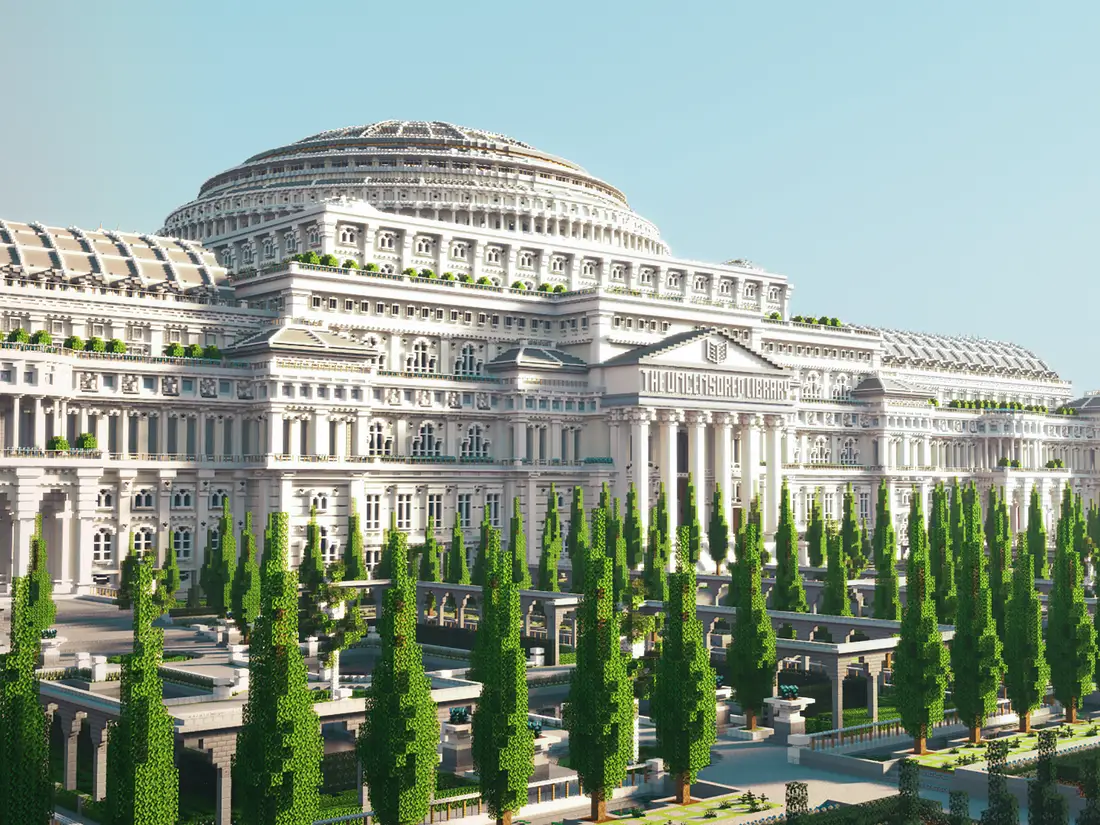
\includegraphics[scale=0.17]{minecraftlibrary.png} \\
\small
\emph{\textbf{Computer Architecture} is a set of rules and methods that describe the functionality, organization, and implementation of computer systems.} \\
\vspace{-10pt}
\flushright -- Wikipedia --
\end{frame}

\begin{frame}{Header Files vs Libraries}
Things that are useful:
\begin{itemize}
\item The ability to call functions defined outside of a source code file.  
\item The ability to pre-compile these functions
\item The ability to share library functions among many programs.
\end{itemize}
These purposes are served by the library system. 
\begin{itemize}
\item \textbf{Header Files} - files containing the prototypes of functions made available by a specific library.  
\item \textbf{Library} - files in which the functions specified in the header file are implemented. There are two main types: \textbf{Static} and \textbf{Dynamic} (see the next slide).
\end{itemize}
Because their functionality is so closely linked, when a person says ``a library'', they usually mean both the library and header file taken in combination.  
\end{frame}

\begin{frame}{Static vs Dynamic Libraries}
\begin{itemize}
\item \textbf{Static} - Derived from the Greek ``statikos'', meaning ``causing to stand''
\begin{itemize}
\item Contain object code linked with a program, which then is integrated into the executable.
\item Included at compile time (i.e., up front)
\item Consequentially, the compiler needs to be able to find it.
\end{itemize}
\item \textbf{Dynamic} - Derived from the Greek ``dunamikos'', meaning ``powerful''
\begin{itemize}
\item Linked to the executable at compile time, but the implementation of the linked function is loaded at \emph{run-time}.  
\item Linking resolves undefined references in the source file
\item May be shared with many programs.  
\end{itemize}
\end{itemize}
\end{frame}

\begin{frame}[fragile=singleslide]{Find it in Your Local Library}
There are two ways to include files.
\begin{lstlisting}[style = C]
#include <stdio.h>
#include "myheader.c"
\end{lstlisting}
\begin{itemize}
\item If the filename is enclosed in quotation marks, gcc will search both the first relative directory of the current file and a preconfigured list of standard system directories.
\item If angle braces are used, \emph{only} the standard system directories are searched.  
\item Technically this means you could use quotes for everything, but by convention, if it's a standard library header, use angle braces.  
\end{itemize}
\end{frame}

\begin{frame}{Header files for miles!}
From the gcc documentation:
\begin{itemize}
\item Header files serve two purposes. 
\begin{itemize}
\item \textbf{System header files} declare the interfaces to parts of the operating system. You include them in your program to supply the definitions and declarations you need to invoke system calls and libraries. 
\item Your own header files contain declarations for interfaces between the source files of your program. Each time you have a group of related declarations and macro definitions all or most of which are needed in several different source files, it is a good idea to create a header file for them. 
\end{itemize}
\end{itemize}
By convention, header files have the *.h file extension.
\end{frame}

\begin{frame}{Some Standard Library Headers}
\center
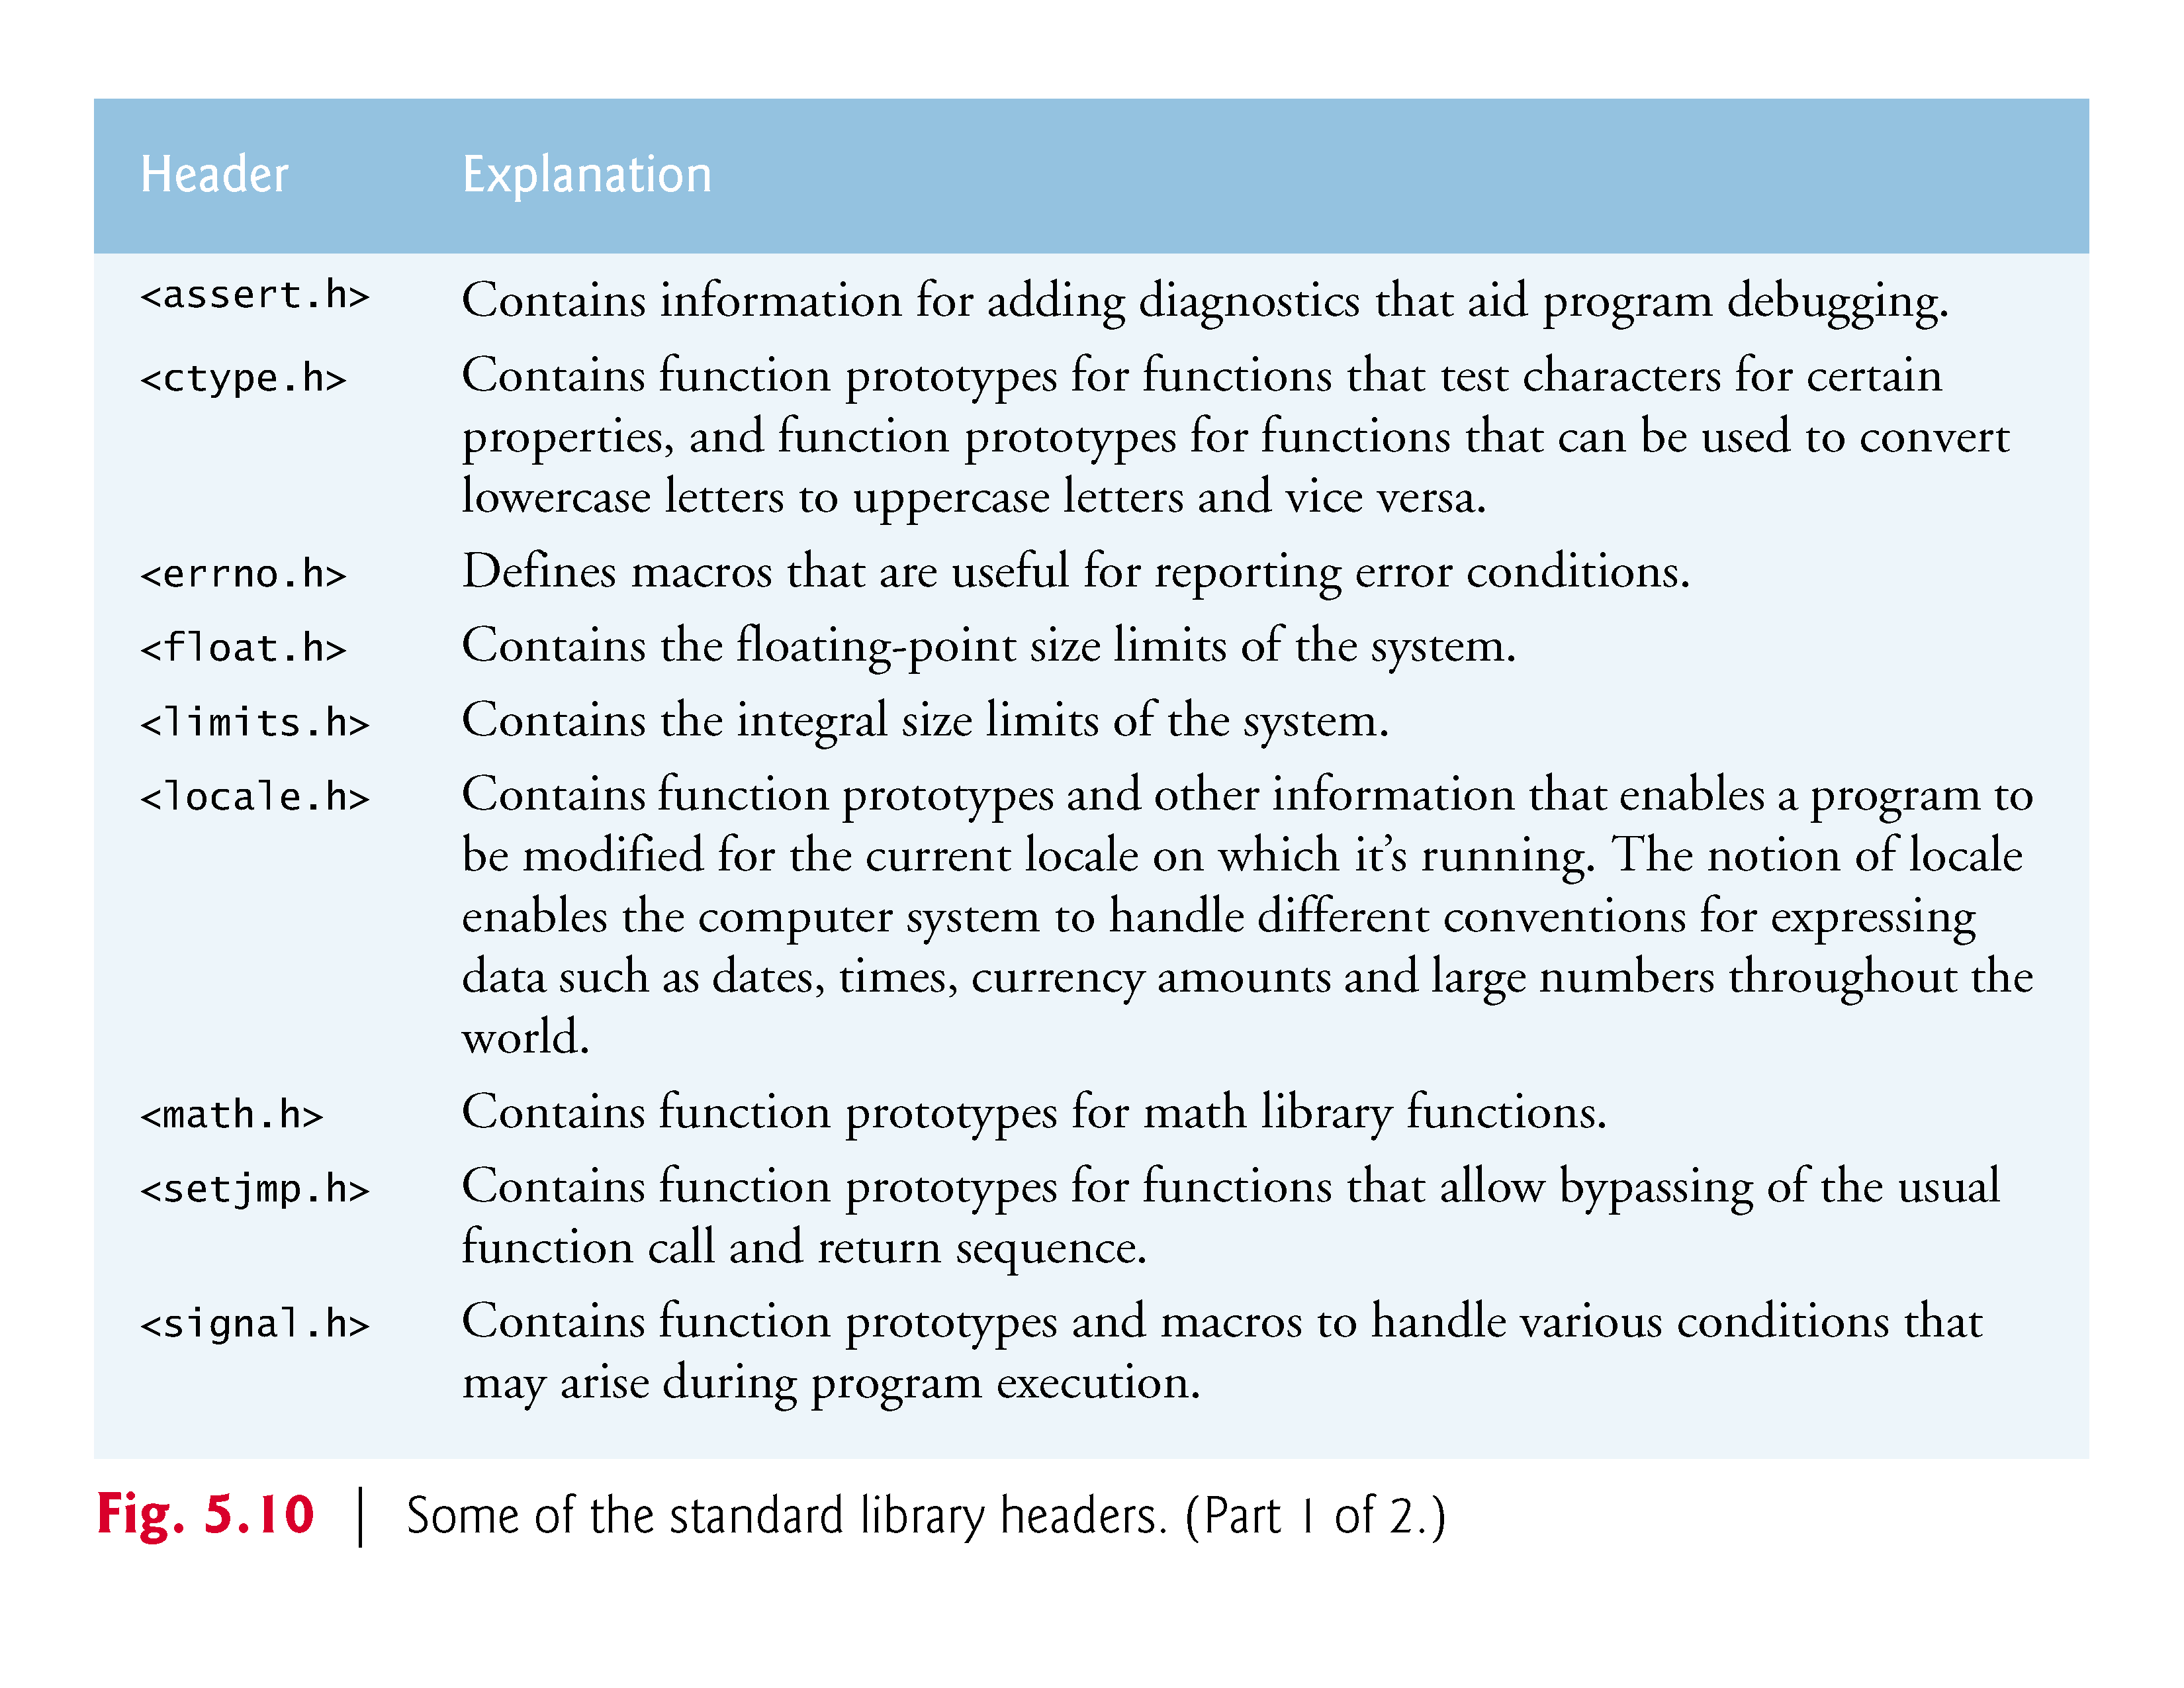
\includegraphics[scale=0.33]{headers1.png}
\end{frame}

\begin{frame}{Some Standard Library Headers}
\center
\includegraphics[scale=0.33]{headers2.png}
\end{frame}

\begin{frame}[fragile=singleslide]{Library Example} 
\begin{lstlisting}[style = C] 
// ><><><><>< top.c ><><><><><
#include <stdio.h>
#include "mylib.h"
int main () {
	int q = max(4,5);
	printf("The maximum is %d\n", q);
}
\end{lstlisting}
\begin{lstlisting}[style = C] 
// ><><><><>< mylib.h ><><><><><
int max (int x, int y);
\end{lstlisting}
\begin{lstlisting}[style = C]
// ><><><><>< mylib.c ><><><><><
int max (int x, int y) {
	if (x > y) { return x;
	} else { return y;
} }
\end{lstlisting}
\end{frame}

\begin{frame}[fragile=singleslide]{Static Compilation}
\begin{itemize}
\item Note that \texttt{lib.c} does not contain a \texttt{main} function!
\end{itemize}
All three of these files are compiled and linked with a single invokation of gcc:
\begin{lstlisting}[style=terminal]
gcc -Wall top.c mylib.c -o top
\end{lstlisting}
\begin{itemize}
\item Runnning gcc on only \texttt{top.c} (omitting \texttt{mylib.c}) will result in an undefined reference, which is an \textbf{error}! 
\end{itemize}
\end{frame}

\begin{frame}{An Alternative Procedure}
It is a stylistic recommendation to write header files for your C files below the top-level.  Especially if they are \textbf{\Large{Large!}}
\begin{itemize}
\item This emulates the way other programming languages use \textbf{packages} and \textbf{modules}.
\end{itemize}
However, the header file may be successfully omitted. In the previous example:
\begin{itemize}
\item Change \texttt{mylib.h} to \texttt{mylib.c} on line 3 of \texttt{top.c}
\item Omit \texttt{mylib.c} from the gcc invokation.
\end{itemize}
\end{frame}

\begin{frame}{Dynamic Libraries}
\begin{itemize}
\item The procedure for creating a dynamic library is operating system dependent, but the goal is to create:
\begin{itemize}
\item A shared object file (\texttt{*.so}) [Mac/Linux]
\item Or a dynamically linked library file (\texttt{*.dll}) [Windows]
\end{itemize}
\item If set up properly, a dynamic library can be used by programs written in \emph{languages other than C!}
\item \textbf{BE WARNED!!} Messing around in your operating system's hidden folders can have \textbf{SERIOUS CONSEQUENCES}! 
\begin{itemize}
\item Never mess around with a computer like this if you don't have your data backed up
\item Don't say your professor didn't warn you! 
\end{itemize}
\end{itemize}
One of the lab activities in this course will require you to create and install a shared object library
\end{frame}


\section[Stack]{Functions: How Do They REALLY Work?}
\begin{frame}{Introducing the \textbf{Call Stack!}}
Have you ever wondered how your computer keeps track of all those function calls?  
\begin{itemize}
\item function calls are stored in your system's \textbf{function call stack} or just \textbf{call stack}, or, reverently, \textbf{The Stack}.
\item The call stack has a fixed, or \emph{static} size.
\item If too many items are added to the call stack, this can result in an error called \textbf{stack overflow} (which what \url{https://stackoverflow.com/} is referencing!)
\item In order to understand the call stack, we need to know some rudimentary data structures!
\end{itemize}
\end{frame}

\begin{frame}{Stacks of Stacks}
\begin{itemize}
\item A \textbf{stack} is a data structure that always returns the most recently added element.
\item This is also known as LIFO (last-in, first-out)
\item There are two primary operations on stacks:
	\begin{itemize}
	\item \textbf{Push} - An element is added to the stack
	\item \textbf{Pop} - The element in the stack that was added most recently is removed from the stack and returned.  
	\end{itemize}
\item The kitchen metaphor is a stack of plates.  How you use a stack of dishes in your cupboard is how your computer uses stacks for data.
\item Undo/redo actions in many programs are also stored in a stack. 
\end{itemize}
\end{frame}

\begin{frame}{A Stack in Operation}
\center
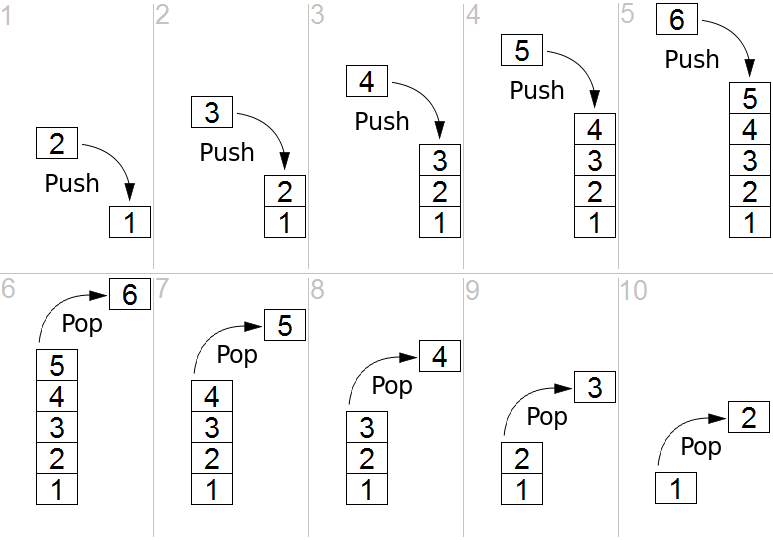
\includegraphics[scale=0.4]{Lifo_stack.png}
\end{frame}

\begin{frame}{Call Stack Functionalities}
The call stack: 
\begin{itemize}
\item enables programs to ``step into'' functions while keeping their place in the program that called the function.
\begin{itemize}
	\item Functions are properly thought of as \emph{sub-programs}
\end{itemize}
\item supports the creation, maintenance, and destruction of each function's local variables.  This is also known as \textbf{namespace}.  
\item keeps track of the return addresses that each function needs to return control to the invoking function.  
\end{itemize}
Think of the previous stack example, but replace the numbers with all of the data necessary to execute a function, including variables.  These are known as \textbf{stack frames}.
\end{frame}

\section[Vars]{Storage Classes, Scoping and a Few Other Things}

\begin{frame}{Pass By Reference vs Pass By Value}
There are two main ways that a programming language will pass data into its functions:
\begin{itemize}
\item \textbf{By Reference} - Perl, VB, Fortran
\begin{itemize}
\item Variables are passed into functions as references to data, rather than the data itself.  
\item Modifying the function argument inside the function will modify the variable passed into the function, within the context of the calling program.  
\end{itemize}
\item \textbf{By Value} - C, Java, Python*
\begin{itemize}
\item The bit values of the variables are passed into functions, rather than references to the memory contained in them.  
\item Modifying an argument does not effect anything outside the function's local context.
\end{itemize}
\end{itemize}
C can pass by reference using pointers, but you have to do the legwork yourself ;-)
\end{frame}

\begin{frame}[fragile=singleslide]{Creating Our Own Types!}
The \texttt{typedef} keyword allows us to define type synonyms:
\begin{lstlisting}[style=C]
typedef unsigned char BYTE; 
\end{lstlisting} 
This allows us to use the new type \texttt{BYTE} anywhere a type must be declared:
\begin{lstlisting}[style=C]
...
	BYTE foo = 0;
...
\end{lstlisting} 
The compiler will swap in the type's synonym at compile time. Type synonyms can be very useful for improving the readability of your code, as they allow for more descriptive type information! \\
\emph{By convention, data types are capitalized!}
\end{frame}


\begin{frame}[fragile=singleslide]{\texttt{enum} With Terror!}
Another way we can define custom types in C is with \textbf{enumerations}
\begin{lstlisting}[style=C]
enum PKMN_STATUS {FNT, SLP, PRZ, PSN, FRZ, BRN, None}; 
\end{lstlisting}
Not only is the type available, but the enumerats may also be used as literals:
\begin{lstlisting}[style=C]
... 
	PKMN_STATUS stat = None;
	if (stat == PSN) {
		hp = hp - hp / 16;
	} 
	if (hp <= 0) {
		stat = FNT;
	}
...
\end{lstlisting}
\end{frame}

\begin{frame}[fragile=singleslide]{\texttt{enum} With Terror! (cont.)}
In reality, each of the enumerats is an alias for a literal bit value.  We can expose these with the following program:
\begin{lstlisting}[style=C]
#include <stdio.h>
enum PKMN_STATUS {FNT, SLP, PRZ, PSN, FRZ, BRN, None}; 
int main() {
	printf("FNT = %d\n", FNT);
	printf("SLP = %d\n", SLP);
	printf("PRZ = %d\n", PRZ);
}
\end{lstlisting}
Just like typedefs, the main purpose of enumerations is \emph{code readability!} 
\end{frame}

% \begin{frame}{Storage Class Modification}
% We can change the scope of identifiers in C using \textbf{Storage Class Modifiers}:
% \begin{itemize} 
% \item \texttt{auto}, \texttt{register}, \texttt{extern}, \texttt{static}
% \end{itemize}
% \center
% \includegraphics[scale=0.3]{Storage-Classes-In-C.png}
% \end{frame}

\section[Arrays]{Arrays: Like Tuples, But More Annoying} % include 6.6, 6.7
\begin{frame}{Arrays: The Simplest Data Structure}
% \center
% \includegraphics[scale=3]{donald_knuth.png} \\
% The joke within the joke is that hat guy imagines he has a choice... \\ 
% -- Your Professor -- 
% \end{frame}

% \begin{frame}{I see data \texttt{Array}ed before me...}
In Python, there are many data structures to choose from:
\begin{itemize}
\item Tuples
\item Lists
\item Dictionaries
\item Sets
\item Strings
\end{itemize}
In C, the only data structure supported natively is the \textbf{Array}.  If you need something more complex than an Array, you have to either find a library defining it or define it yourself. 
\end{frame}

\begin{frame}{So what is an \texttt{Array}?}
An array is a contiguous segment of memory, which may be accessed via linear indexing.
\begin{itemize}
\item All elements of an array have the same type.
\item Arrays use \textbf{zero-indexing}.
\item Arrays are \emph{static}
\begin{itemize}
\item The size of an array does not change during execution
\item This means that the size of the array \emph{must} be known at the time of declaration.  
\item There are ways of getting around this, but not without pointers (which we'll be talking about soon...)
\end{itemize}
\end{itemize}
\end{frame}

\begin{frame}[fragile=singleslide]{Syntax, my friends!}
An array is declared in the following manner:
\begin{lstlisting}[style=C]
int c[x];
\end{lstlisting}
\begin{itemize}
\item Note, that $x$ must be either an integer literal or an expression which evaluates to an integer. 
\begin{itemize}
\item This rule applies to array indexing as well as declaration.
\end{itemize} 
\item On declaration, an array is filled with \emph{junk data!}
\end{itemize}
Arrays may be indexed using the array index operator:
\begin{lstlisting}[style=C] 
c[7] = 5;
\end{lstlisting} 
\begin{itemize}
\item Binds at the same level as function calls (so very tightly)
\item As we'll see later, the index operator is syntactic sugar for some pointer operations.
\end{itemize}
\end{frame}

\begin{frame}[fragile=singleslide]{Pretty Printing Arrays}
\begin{lstlisting}[style=C] 
#include <stdio.h>
int main () {
	int c[(6+6)];
	float bar[] = {0.0, 0.1, 0.2, 0.3};
	printf("%d\n", c);
	printf("%p\n", c);
	printf("[");
	for (int i = 0; i < 12; i++) {
		if (i < 11) {
			printf("%d, ", c[i]);
		} else {
			printf("%d]\n", c[i]);
		}
	}
}
\end{lstlisting} 
\end{frame}

\begin{frame}{Pretty Printing Arrays (Visualization)}
\center
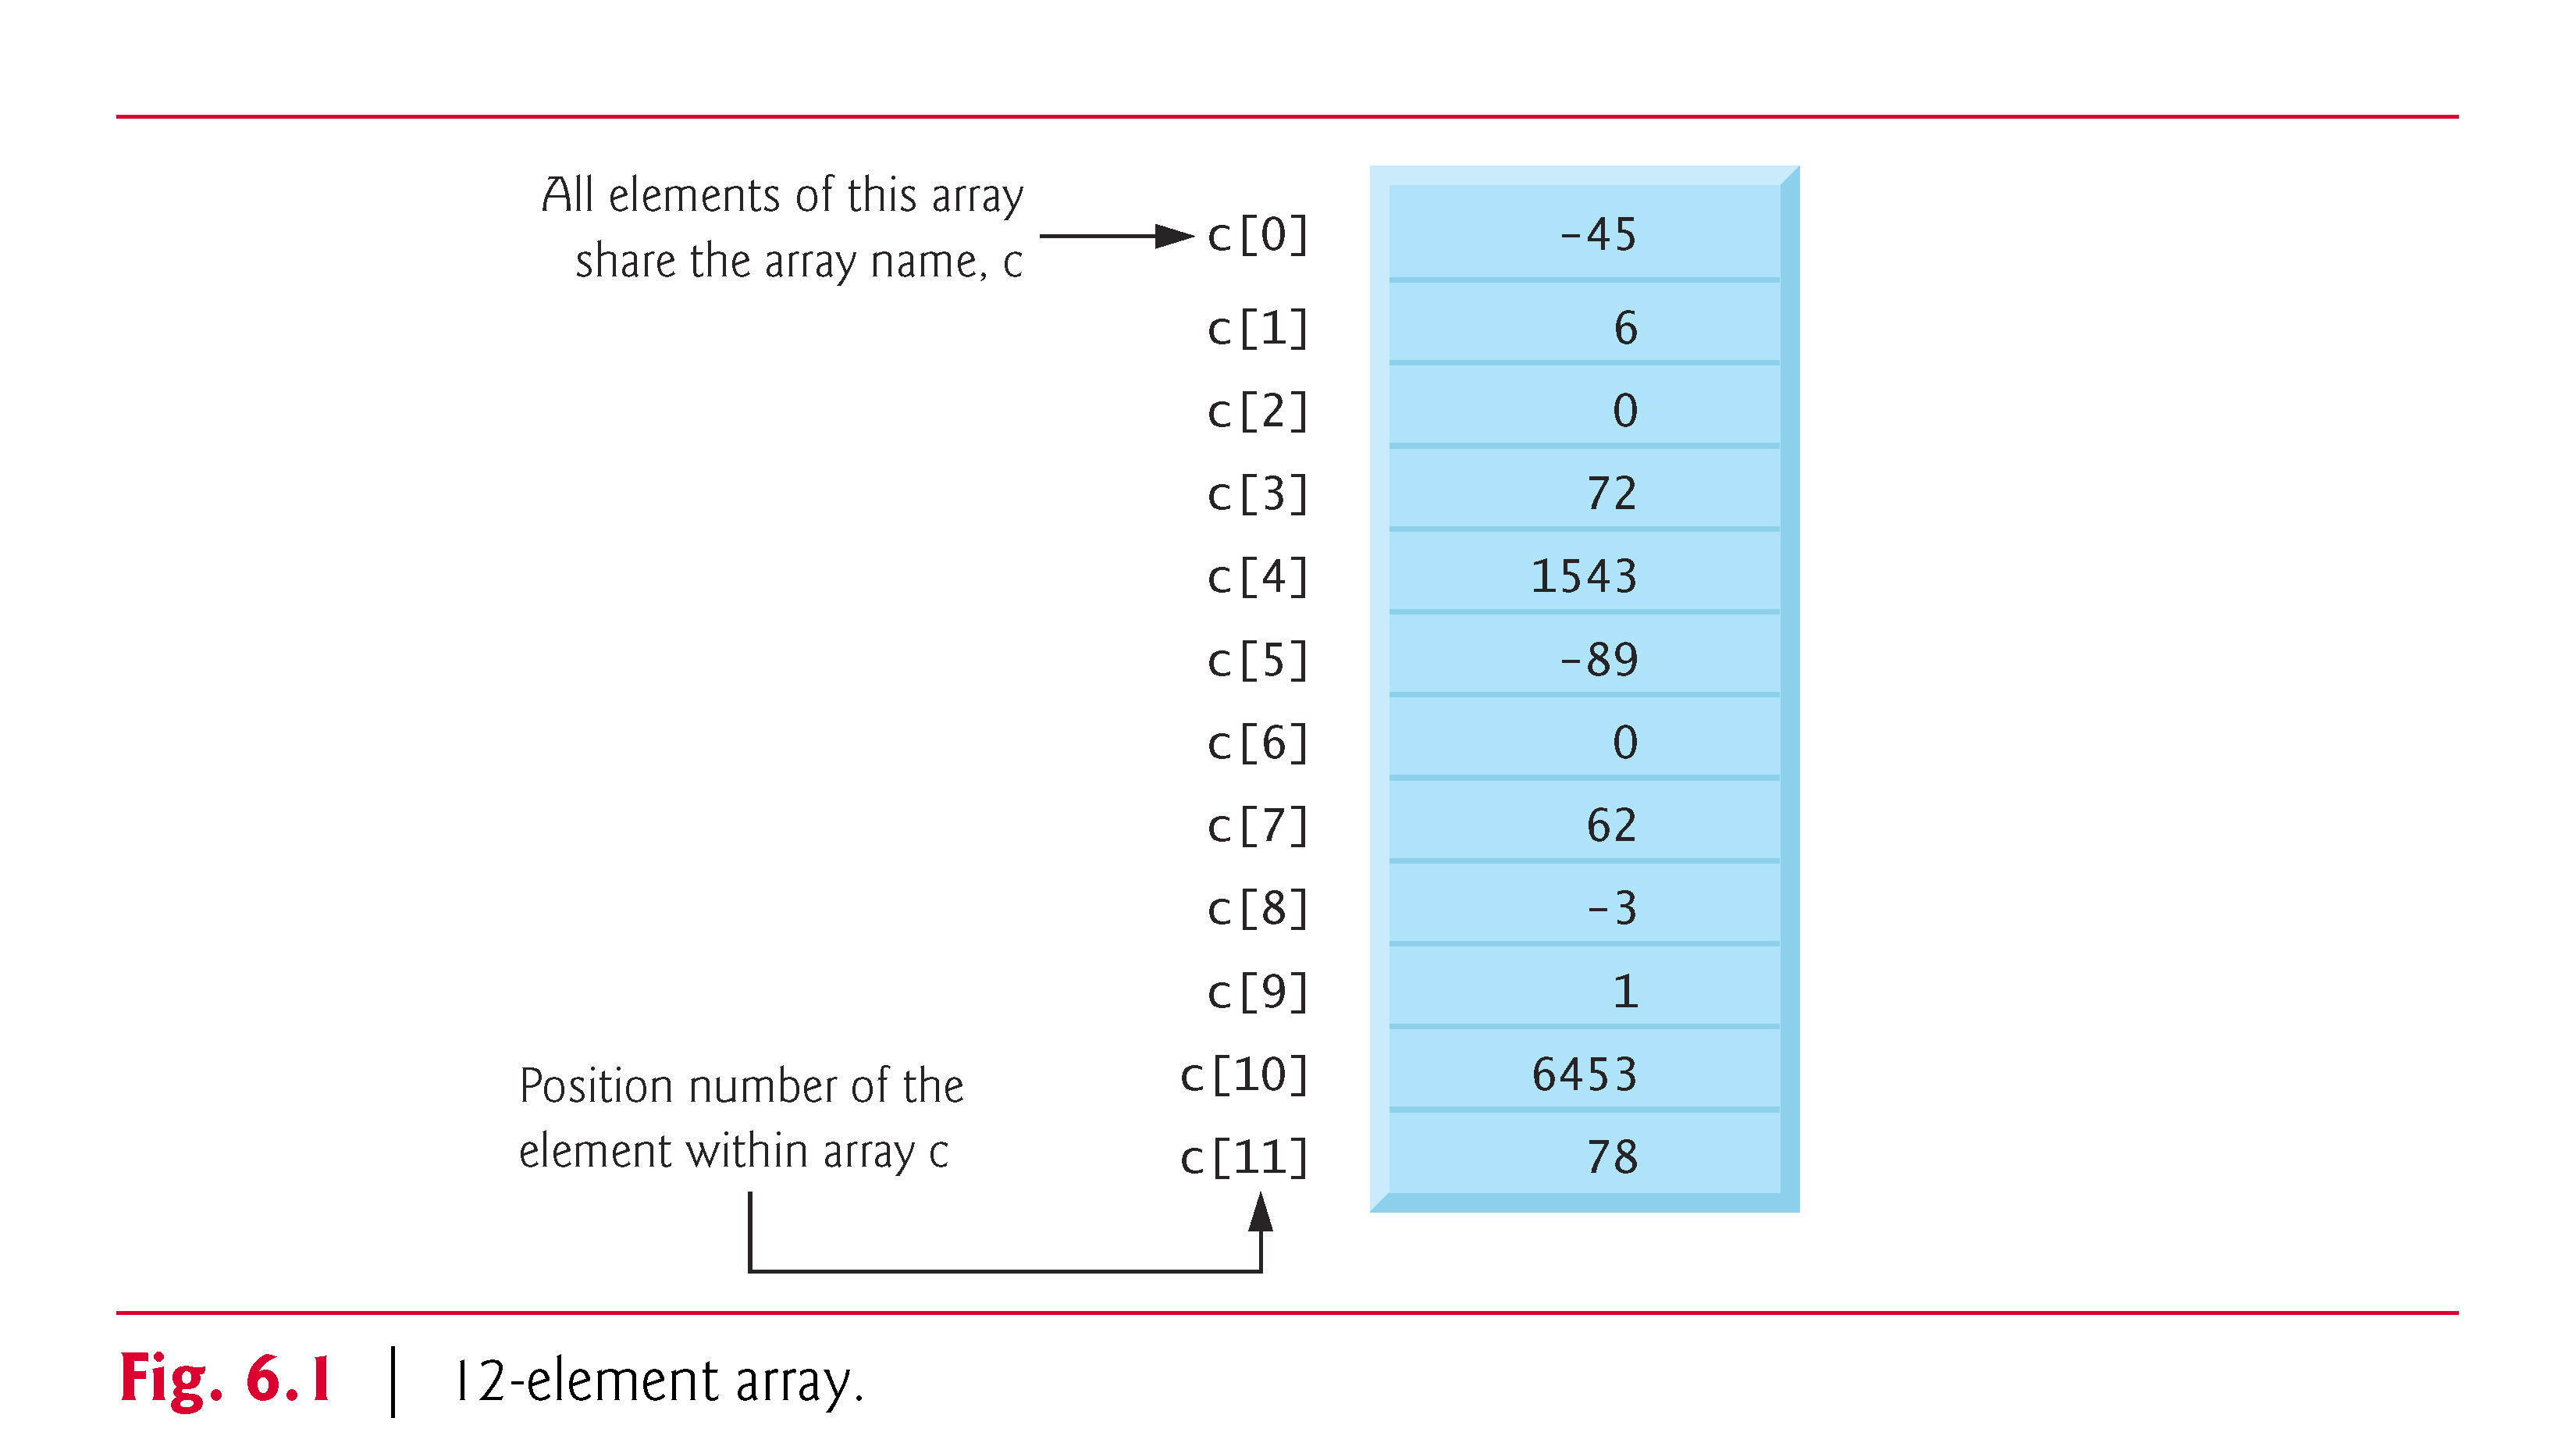
\includegraphics[scale=0.1]{array.png}
\end{frame}

\begin{frame}[fragile=singleslide]{Pretty Printing Arrays (output)}
Compiler Warnings:
\begin{lstlisting}[style=terminal]
In function 'main':
warning: format '%d' expects argument of type 'int', 
  but argument 2 has type 'int *'
  printf("%d\n", c);
          ~^     ~~~
          %ls
\end{lstlisting}
Output:
\hrule
\begin{lstlisting}[style=terminal]
-1506989472
0x7ffca62d2a60
[1, 0, 56797197, 22077, 997394928, 32685, 0, 0, 
  56797120, 22077, 56796656, 22077]
\end{lstlisting}
\end{frame}

\begin{frame}{Pretty Printing Arrays (Analysis)}
Just like with a lot of things in C, there are no free lunches! 
\begin{itemize}
\item You can't print a whole array just by passing the array's name to \texttt{printf} as the array identifier is really a \textbf{memory address}, or \textbf{pointer}.
\end{itemize}
Initialization!
\begin{itemize}
\item An uninitialized array is full of garbage data! 
\item To initialize an array, provide a comma separated series of type-correct literals or expressions, delimited with curly braces! 
\item If the initializer is smaller than the declared memory, C backfills with zeros!
\item If you initialize the array, you may omit specifying the size (the size of the initializing array will be used).
\end{itemize}
\end{frame}

\begin{frame}[fragile=singleslide]{Arrays and Functions}
Consider the following function prototype:
\begin{lstlisting}[style=C]
int* myFun (const int input[]);
\end{lstlisting}
\begin{itemize}
\item \texttt{input} is declared as an array by the inclusion of \texttt{[]}
\begin{itemize}
\item \texttt{int*} is also valid.
\end{itemize}
\item \texttt{int*} tells us that this function returns an \textbf{integer pointer}
\begin{itemize}
\item Arrays in C are syntactic sugar for pointers.
\end{itemize}
\item the \texttt{const} term locks the pointer so that it can't be modified.  This essentially makes it ``read-only''
\begin{itemize}
\item This will prevent any of the array's elements from being modified, as well as the value of the pointer.  
\item If you want to be able to modify the array, just leave out the \texttt{const} keyword.
\item You can do this with any argument, not just arrays!
\end{itemize}
\end{itemize}
\end{frame}

\begin{frame}[fragile=singleslide]{\texttt{sizeof}}
In Python, we have the \texttt{len()} function to quickly and easily tell us how large our data structures are.  
\begin{itemize}
\item The equivalent fuction in C is \texttt{sizeof()}, but as with most things in C, it's a bit more complicated.
\item \texttt{sizeof()} returns the size \emph{in bytes} that the provided argument was declared with.   
\item \texttt{sizeof()} may be used on variables of any type, not just arrays.
\item Accordingly, the \emph{declared} length of an array is equal to the size of the array (in bytes) divided by the size of any element of the array (in bytes):
\begin{lstlisting}[style=C]
int foo[] = {1,2,3,4,5,6}
length = sizeof(foo) / sizeof(foo[0]);
\end{lstlisting}
\end{itemize}
\end{frame}

\begin{frame}[fragile=singleslide]{Accessing Higher Dimensions}
Linear arrays are all well and good, but what if I need to represent a matrix? 
\begin{lstlisting}[style=C]
// Declaring a 2D array
int foo[][] = {{1, 2}, {3, 4}};
// Declaring a 3D array
int bar[5][5][5];
\end{lstlisting}
\begin{itemize}
\item Dimensionality is indicated by the number of square braces following the identifier.
\item These are correctly thought of as \emph{arrays of arrays}.
\item Providing $n-k$ indexes to an $n$ dimensional array will produce a $k$ dimensional array.
\end{itemize}
\end{frame}

\section[String]{Strings are Character Arrays!} 
\begin{frame}{Strings are Character Arrays!}
\center
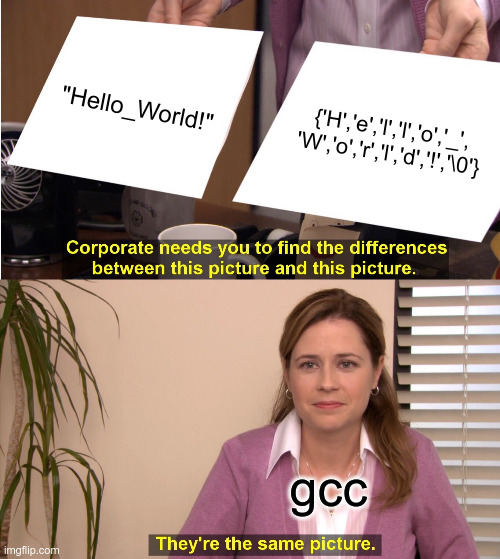
\includegraphics[scale=0.3]{charArrays.jpg}
\end{frame}

\begin{frame}[fragile=singleslide]{Character Arrays, not Character Sheets...}
As it turns out, C handles strings as \textbf{character arrays.} Consider the following declarations:
\begin{lstlisting}[style=C]
char foo[] = "bar";
\end{lstlisting}
\texttt{foo} will be written into memory as:
\begin{center}
\includegraphics[scale=0.5]{string.png}
\end{center}
If we specify a size of ten,
\begin{lstlisting}[style=C]
char foo[10] = "bar"
\end{lstlisting}
 we get the following:
 \begin{center}
 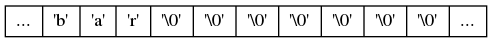
\includegraphics[scale=0.5]{string2.png}
 \end{center}

\end{frame}

\begin{frame}[fragile=singleslide]{String Things}
\begin{itemize}
\item \texttt{string} isn't even a keyword in C! 
\item Character arrays may be indexed, just like regular arrays.
\item String literals are always terminated by the \textbf{null character} implicitly!
\item All strings must be null terminated.
\item We can receive strings directly from \texttt{scanf} using the\texttt{\%s} format specifier.
\begin{lstlisting}[style=C]
scanf("%14s", foo);
\end{lstlisting}
\item By inserting a number, the format specifier may even be used to limit the number of characters that get copied into the character array.  
\item \texttt{foo} is actually a \textbf{pointer}, so we don't need the address-of operator \texttt{\&} in scanf. \texttt{foo} is already a memory address.
\end{itemize}
\end{frame}

\begin{frame}{Overflow Attacks!}
A common form of security vulnerablility in C and C++ programs is \textbf{array overflow}. 
\begin{itemize}
\item Arrays are replaced with pointer arithmetic by the compiler, with no bounds checking!  
\item If you tell C to write 100 characters into a 50 character array, it will happily do so! 
\item The extra 50 characters will be written into the memory that comes after the character array.
\item This can overwrite all kinds of useful things, like other variables.  If the character array is stored in the stack, function call informaton can also be vulnerable.  
\end{itemize}
The moral of the story is that you should always limit the things you write into an array to the size of the array MANUALLY! 
\end{frame}

\begin{frame}[fragile=singleslide]{Smash that Stack!}
\begin{lstlisting}[style = C]
#include <stdio.h>

int main() {
	char query[10];
	printf("Enter A Query : ");
	scanf("%s", query);
	printf("The query is %s\n", query);
}
\end{lstlisting}
\hrule
\begin{lstlisting}[style=terminal]
Enter A Query : jjjjjjjjjjjjjjjjjjjjjjjjjjjjjjj
The query is jjjjjjjjjjjjjjjjjjjjjjjjjjjjjjj
*** stack smashing detected ***: <unknown> terminated
	Aborted (core dumped)
\end{lstlisting}
\end{frame}

\section[Acknowledge]{Acknowledge}
\begin{frame}{Acknowledge}
\center
\vspace{8em}
The contents of these slides were liberally borrowed (with permission) from slides from the Summer 2021 offering of 1XC3 (by Dr. Nicholas Moore).  
\end{frame}

\end{document}
